\section{Техническое задание}
\subsection{Основание для разработки}

Основанием для разработки является задание на выпускную квалификационную работу бакалавра "<Разработка системы управления содержимым веб-сайтов">.

\subsection{Цель и назначение разработки}

Разрабатываемая программно-информационная система предназначена для совместного создания и управления веб-сайтами, не требуя от пользователей навыков программирования и веб-разработки. 

Задачами данной разработки являются:
\begin{itemize}
	\item разработка пользовательского интерфейса (административной панели) системы;
	\item разработка структуры базы данных для хранения информации о сущностях системы;
	\item разработка серверной части системы;
	\item разработка визуального редактора контента;
	\item реализация управления пользователями и правами доступа;
	\item реализация возможности выбора и применения различных тем (шаблонов) веб-сайта;
	\item реализация возможности совместной работы нескольких пользователей над контентом;
	\item организация хранилища медиафайлов.
\end{itemize}

\subsection{Требования к программной системе}
\subsubsection{Требования к данных программной системы}

Входными данными для программной системы являются:
\begin{itemize}
	\item содержимое страниц и записей (постов): текст, медиафайлы;
	\item категории и теги для организации записей (постов);
	\item метаданные для страниц: заголовок, описание, ключевые слова;
	\item пользовательские данные: регистрационная информация (имя пользователя, пароль);
	\item файлы темы (шаблона) оформления сайта;
	\item настройки и параметры: название, адрес сайта.
\end{itemize}

Выходными данными для программной системы будут:
\begin{itemize}
	\item отображение данных в виде веб-страниц;
	\item вывод содержимого медиафайлов на веб-страницах;
	\item использование тем (шаблонов) для оформления содержимомого страниц сайта;
	\item применение настроек и параметров к сайту.
\end{itemize}

\subsubsection{Функциональные требования к программной системе}

На основании анализа предметной области в разрабатываемой программной системе должны быть реализованы следующие функции:
\begin{enumerate}
	\item Аутентификация и авторизация пользователей.
	\item Управление веб-страницами.
	\item Управление записями (постами).
	\item Управление категориями и тегами записей (постов).
	\item Управление меню и навигацией на сайте.
	\item Управление темой (шаблоном) сайта.
	\item Управление пользователями.
	\item Управление настройками сайта.
\end{enumerate}

На рисунке \ref{usecase:image} представлены функциональные требования к системе в виде диаграммы прецедентов нотации UML.

\begin{figure}[ht]
	\center{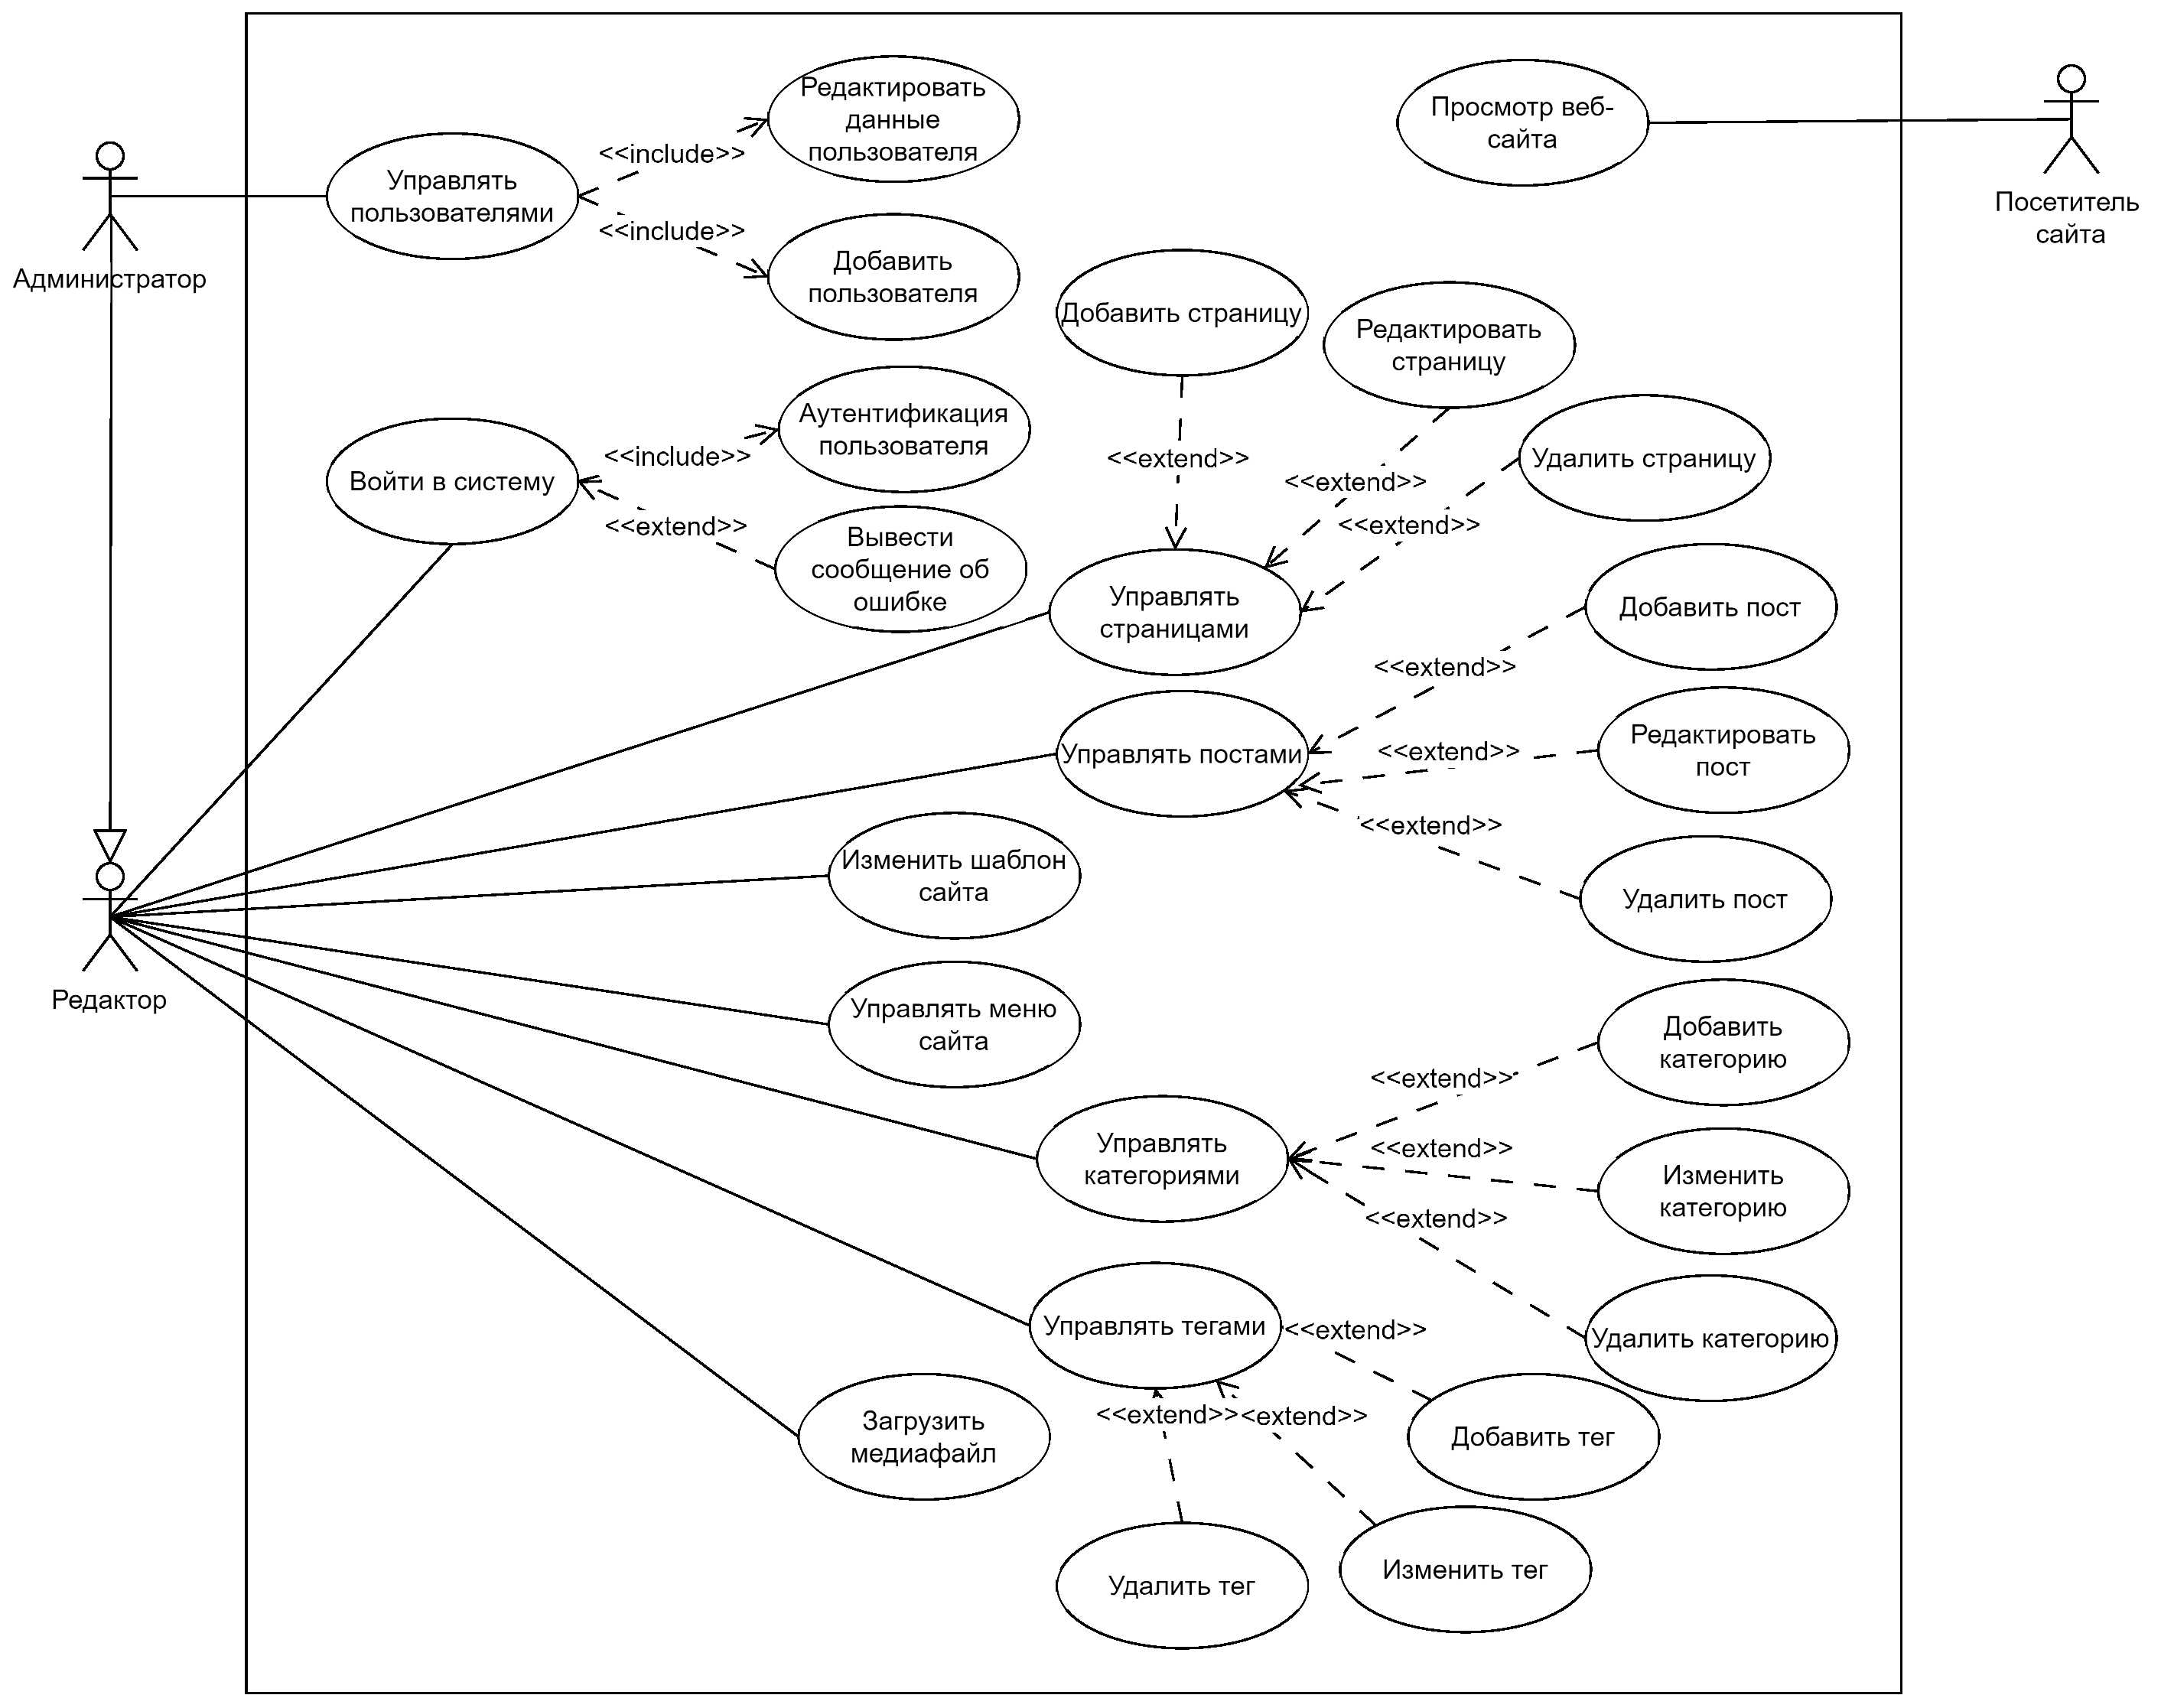
\includegraphics[width=1\linewidth]{usecase}}
	\caption{Диаграмма прецедентов}
	\label{usecase:image}
\end{figure}

\subsubsection{Моделирование вариантов использования}
\paragraph{Вариант использования <<Войти в систему>>}
Заинтересованные лица и их требования: пользователь хочет поулчить доступ к административной панели сайта.

Предусловие: пользователь зарегистрирован в системе и знает свои данные для входа (логин и пароль).

Постусловие: система авторизует пользователя в соответствии с его ролью.

Основной успешный сценарий:
\begin{enumerate}
	\item Пользователь вводит адрес административной панели сайта в браузере для перехода на страницу входа в систему.
	\item Пользователь вводит логин и пароль.
	\item Система проверяет корректность введенных данных и аутентифицирует пользователя.
	\item Пользователь перенаправляется на главную страницу административной панели сайта.
\end{enumerate}

\paragraph{Вариант использования <<Управлять пользователями>>}
Заинтересованные лица и их требования: администратор хочет управлять учетными записями пользователей и их ролями в системе.

Предусловие: пользователь авторизован и имеет права администратора.

Постусловие: изменения в учетных записях пользователей сохранены в системе.

Основной успешный сценарий:
\begin{enumerate}
	\item Администратор открывает раздел управления пользователями.
	\item Администратор выбирает действие (создание, редактирование, удаление пользователя).
	\item Администратор вводит необходимую информацию о пользователе.
	\item Система сохраняет изменения и обновляет список пользователей.
\end{enumerate}

\paragraph{Вариант использования <<Управлять страницами сайта>>}
Заинтересованные лица и их требования: пользователь хочет управлять страницами сайта.

Предусловие: пользователь авторизован в системе и имеет соответствующие права доступа.

Постусловие: изменения сохранены и отображаются на сайте.

Основной успешный сценарий:
\begin{enumerate}
	\item Пользователь открывает раздел управления страницами.
	\item Пользователь создает новую страницу или выбирает существующую для редактирования.
	\item Пользователь переходит в режим редактирования страницы.
	\item Пользователь добавляет новый или выбирает существующуй элемент страницы для редактирования.
	\item Пользователь вносит необходимые изменения в содержимое элемента.
	\item Пользователь вносит необходимую информацию о странице (название, URL, метаданные).
	\item Пользователь сохраняет изменения.
\end{enumerate}

\paragraph{Вариант использования <<Управлять постами>>}
Заинтересованные лица и их требования: пользователь хочет упралять постами.

Предусловие: пользователь авторизован в системе и имеет соответствующие права доступа.

Постусловие: изменения в постах сохранены и отображаются на соответствующей странице сайта.

Основной успешный сценарий:
\begin{enumerate}
	\item Пользователь открывает раздел управления постами.
	\item Пользователь создает новый пост или выбирает существующий для редактирования.
	\item Пользователь вносит необходимые изменения в текст, заголовок, метаданные и т. д..
	\item Пользователь сохраняет или публикует новый пост.
\end{enumerate}

\paragraph{Вариант использования <<Управлять категориями и тегами постов>>}
Заинтересованные лица и их требования: пользователь хочет управялть категориями и тегами постов.

Предусловие: пользователь авторизован в системе и имеет соответствующие права доступа.

Постусловие: изменения в категориях и тегах сохранены и применены к соответствующим постам.

Основной успешный сценарий:
\begin{enumerate}
	\item Пользователь открывает подраздел управления категориями и тегами постов.
	\item Пользователь создает новую категорию/тег или редактирует существующие.
	\item Пользователь присваивает их соответствующим постам.
	\item Система сохраняет изменения и реорганизует отображение постов.
\end{enumerate}

\paragraph{Вариант использования <<Управлять меню и навигацией сайта>>}
Заинтересованные лица и их требования: пользователь хочет управялть навигационным меню сайта.

Предусловие: пользователь авторизован в системе и имеет соответствующие права доступа.

Постусловие: изменения в меню сохранены и отображаются на сайте.

Основной успешный сценарий:
\begin{enumerate}
	\item Пользователь открывает раздел управления меню и навигацией сайта.
	\item Пользователь создает новый пункт меню, редактирует существующие.
	\item Пользователь изменяет их порядок или структуру.
	\item Пользователь сохраняет изменения.
\end{enumerate}

\paragraph{Вариант использования <<Изменить шаблон>>}
Заинтересованные лица и их требования: пользователь хочет изменить шаблон дизайна сайта.

Предусловие: пользователь авторизован в системе и имеет соответствующие права доступа.

Постусловие: выбранный шаблон применен к страницам сайта.

Основной успешный сценарий:
\begin{enumerate}
	\item Пользователь открывает раздел управления шаблонами административной панели.
	\item Пользователь выбирает одну из доступных тем (шаблонов).
	\item Пользователь нажимает соответствующую кнопку для активации темы (шаблона).
	\item Система сохраняет изменения и обновляет шаблон сайта.
\end{enumerate}

\paragraph{Вариант использования <<Загрузить медиафайл>>}
Заинтересованные лица и их требования: пользователь хочет иметь возможность загрузки и удаления медиафайлов.

Предусловие: пользователь авторизован в системе и имеет соответствующие права доступа.

Постусловие: медиафайлы загружены и доступны для использования на сайте.

Основной успешный сценарий:
\begin{enumerate}
	\item Пользователь открывает раздел управления медиафайлами административной панели.
	\item Пользователь нажимает соответствующую кнопку для загрузки файла и выбирает файл.
	\item Система сохраняет файл в соответствующую папку на сервере.
\end{enumerate}

\subsubsection{Требования пользователя к интерфесу программной системы} \label{interface_requirements}
Интрефейс пользователя административной панели разрабатываемой системы управления содержимым должен включать следующие компоненты:
\begin{enumerate}
	\item Навигационное меню.
	\item Редактор контента.
	\item Интерфейс управления страницами сайта.
	\item Интерфейс управления записями (постами).
	\item Интерфейс управления виджетами.
	\item Интерфейс управления меню и навигацией на сайте.
	\item Интерфейс управления пользователями.
	\item Интерфейс управления темами (шаблонами) сайта.
	\item Интерфейс управления медиафайлами.
\end{enumerate}

Навигационное меню предназначено для перемещения по разделам и функциям CMS.

Интерфейс редактора контента включает панели инструментов с кнопками для форматирования текста, добавления ссылок, вставки изображений, видео, таблиц и т. д.

Интерфейс управления страницами сайта отображает список страниц сайта, включает кнопки для создания, редактирования, удаления страниц, поля для ввода данных страницы при добавлении или редактировании страницы.

Интерфейс управления записями (постами) отображает список записей, включает кнопки для создания, редактирования, удаления записей, поля для ввода данных при добавлении или редактировании записи.

Интерфейс управления медиафайлами отображает список загруженных файлов и включает кнопки для загрузки, просмотра, редактирования и удаления медиафайлов.

Интерфейс управления пользователями отображает список пользователей системы и включает кнопки для создания, редактирования и удаления учетных записей пользователей.

Интерфейс управления шаблонами отображает список доступных тем (шаблонов) и кнопку для активации выбранной темы.

Интерфейс управления меню и навигацией включает возможность управления навигационными меню и ссылками на страницы.

При реализации пользовательского интерфейса должны быть использованы следующие технологии:
\begin{itemize}
	\item язык разметки веб-страниц HTML -- для описания структуры страниц веб-интерфейса;
	\item каскадные таблицы стилей СSS -- для стилизации элементов интерфейса;
	\item язык программирования JavaScript -- для создания интерактивного интерфейса;
	\item библиотека jQuery языка программирования JavaScript -- для обмена данными с сервером и обновления элементов интерфейса.
\end{itemize}

\subsection{Нефункциональные требования к программной системе}
\subsubsection{Требования к надежности}
В приложении не должно возникать критических ошибок, приводящих к экстренному завершению работы.
\subsubsection{Требования к программному обеспечению}
Для реализации программной системы должены быть использованы следующие технологии:
\begin{itemize}
	\item язык программирования PHP -- для разработки серверной части;
	\item СУБД MySQL -- для хранения данных и организации данных;
	\item веб-сервер Apache HTTP Server -- для обработки клиентских запросов.
\end{itemize}

\subsubsection{Требования к аппаратному обеспечению}
Для работы приложения, установленного на компьютер, необходимо дисковое пространство не менее 100 Мб, свободная оперативная память в размере не менее 1024 Мб, видеокарта с не менее 1024 Мб видеопамяти, клавиатура, мышь, установленная операционная система Windows, macOS или Linux, архитектура процессора х86 (Windows) или x64 (Windows, macOS, Linux). 

Для доступа к административной панели системы, потребуется браузер Google Chrome, Mozilla Firefox или Microsoft Edge.
\subsubsection{Требования к оформлению документации}
Разработка программной документации и программного изделия должна производиться согласно ГОСТ 19.102-77 и ГОСТ 34.601-90. Единая система программной документации.